\documentclass[../summary.tex]{subfiles}

\begin{document}
\section{Raw materials and circular economy}
\subsection{Introduction}	
\subsubsection{What are resources}
	
Our prosperity relies on easy access to abundant raw materials, with global demand exceeding 100 billion tonnes annually and predicted to double by 2060. Raw materials, substances or resources processed for product creation, are sourced from the earth's crust, nature, and recycled waste in the economy or technosphere. \\
\\
Examples of raw materials from the lithosphere or earth crust are fossil oil and gas, iron ore, bauxite as raw material for aluminium, minerals such as sand or marble, lithium brines, and so on. Metals are often found in ores with varying concentrations, and their distribution is uneven globally. Biomass, derived from nature, includes plant-based and animal-derived materials. Secondary raw materials, extracted from recycled waste, vary in extraction rates, e.g., lead at 70\%, while lithium remains below 1\%. Despite recycling efforts, 88 to 94\% of materials in new products still come from primary resources. \\
\\
Raw material sources span the litho-, bio-, and technosphere. The industrial metabolism concept likens the economy's material processes to the human body's metabolism, providing insight into material management, waste, and emissions for sustainable improvements.

\subsubsection{Case: Electric car}

The ongoing effort to combat climate change includes a significant focus on the energy transition, with a key aspect being the widespread adoption of electric vehicles (EVs). The transition is evident in the rapid increase in EV sales, accounting for 14\% of new car sales in 2022, up from 9\% in 2021 and 5\% in 2020. Figure \ref{fig:electriccarsales} depicts a substantial rise in electric car sales, reaching an estimated 14 million in 2023, with 8 million sold in China.

\begin{figure}[H]
	\centering
	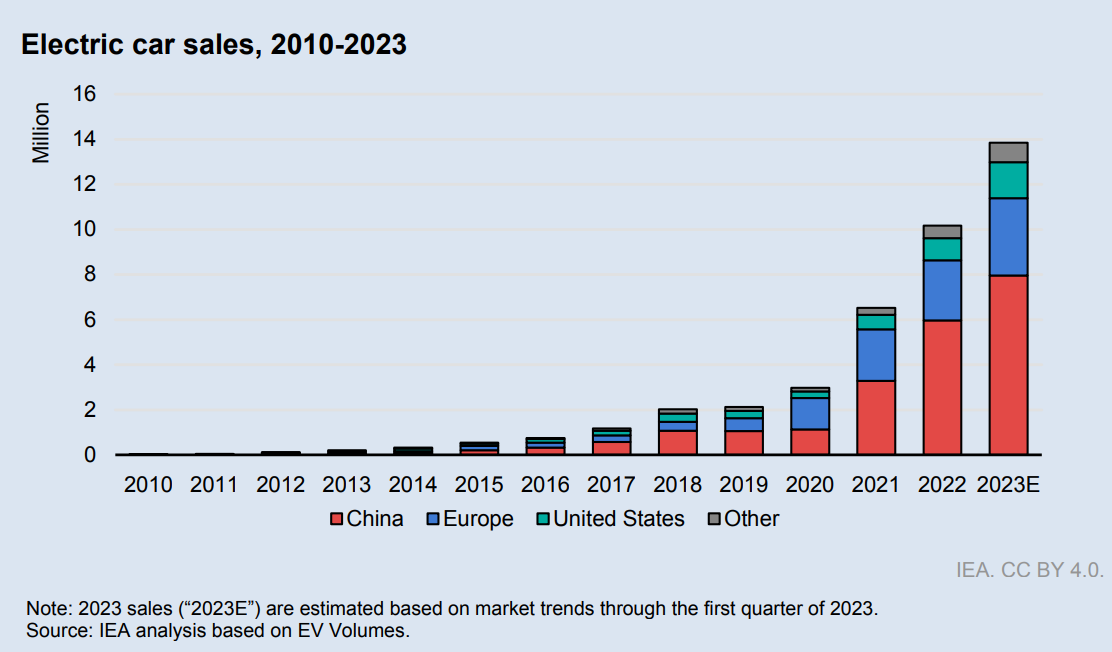
\includegraphics[width=0.7\linewidth]{../images/Electric_car_sales}
	\caption{Electric car sales between 2010 and 2023}
	\label{fig:electriccarsales}
\end{figure}
\ \\
The shift to EVs brings about a change in the materials used, replacing combustion engines with catalysts containing Pt, Pd, and Rh with electric motors requiring copper and neodymium magnets (NdFeB). Power is supplied by Li-ion batteries, raising concerns about the availability of materials to meet the growing demand. Questions arise regarding the duration of lithium availability for Li-ion batteries and the overall environmental impact of EVs compared to traditional combustion engine vehicles. Additionally, considerations about battery recycling and recyclability play a crucial role in evaluating the sustainability of electric vehicles.

\subsection{title}



\end{document}